\PassOptionsToPackage{quiet}{fontspec}
\documentclass[12pt]{article}
\usepackage[a4paper, total={6.5in, 10in}]{geometry}
\usepackage{amsmath}
\usepackage{fontspec}
\usepackage{ctex}
\usepackage{fontawesome5}
\usepackage{xcolor}
\usepackage{booktabs}
\usepackage{multicol}
\usepackage{graphicx}
\usepackage{float}
\usepackage{listings}
\usepackage{svg}
\usepackage{emoji}
\setemojifont{Twemoji Mozilla}  
\usepackage{tikz}
\usepackage{tcolorbox}
\tcbuselibrary{skins}


\newcommand{\scale}[2]{%
    \scalebox{#1}[#1]{#2}}
\lstset{
    backgroundcolor=\color{orange!10},
    numbers=left,
    numbersep=8pt,
    basicstyle=\tt,
    keywordstyle=\color{purple}\bfseries,
    identifierstyle=\color{brown!80!black},
    commentstyle=\color{gray},
    showstringspaces=true,
    frame=tb,
    % frameround=tttt,
}
% 一个tcolorbox盒子
\newtcolorbox{warning}[1][]{%
    enhanced,
    before skip=2mm, after skip=3mm,
    boxrule=0.4pt,left=5mm, right=2mm,top=1mm,bottom=1mm,
    colback=yellow!50, colframe=yellow!20!black,
    sharp corners,rounded corners=southeast,arc is angular,arc=3mm,
    underlay={%
        \path[fill=tcbcolback!80!black] ([yshift=3mm]interior.south east)--++(-0.4,-0.1)--++(0.1,-0.2);
        \path[draw=tcbcolframe,shorten <=-0.05mm,shorten >=-0.05mm] ([yshift=3mm]interior.south east)--++(-0.4,-0.1)--++(0.1,-0.2);
        \path[fill=yellow!50!black,draw=none] (interior.south west) rectangle node[white]{\Huge\bfseries !} ([xshift=4mm]interior.north west);
    },
    drop fuzzy shadow,#1
}


% 1.西文字体
\newfontfamily{\Nainao}[Path=./Fonts/]{NaiNao.ttf}
\newfontfamily{\AlphaProta}[Path=./Fonts/]{AlphaProta.otf}
\newfontfamily{\Meslo}[Path=./Fonts/]{MesloLGL.ttf}
\newfontfamily{\ComicBlue}[Path=./Fonts/]{comic.ttf}[Color=blue]
\newfontfamily{\ComicA}[Path=./Fonts/]{comic.ttf}
\newfontfamily{\ComicB}[Path=./Fonts/]{comic.ttf}[
    BoldFont=comicbd.ttf,
    ItalicFont=comici.ttf,
    BoldItalicFont=comicz.ttf
]
\newfontfamily{\Girlanything}[Path=./Fonts/]{Girlanything.otf}
\newfontfamily{\Thei}[Path=./Fonts/]{TheiFont.otf}
\newfontfamily{\FathonyKing}[Path=./Fonts/]{FathonyKing.otf}

% 2.中文字体
\setCJKfamilyfont{PinRu}[Path=./Fonts/]{PinRu.ttf}
\setCJKfamilyfont{AutoF}{FZSTK.TTF}[AutoFakeBold, AutoFakeSlant]
% 3.表情包字体
\newfontfamily{\emojifonta}[Path=./Fonts/]{seguiemj.ttf}


\title{\Girlanything Font Config Tutorial}
\author{Eureka}
\date{}
% 目录重命名
\renewcommand{\contentsname}{\Thei Contents}
\begin{document}
\thispagestyle{empty}
\maketitle
\begin{center}
    \tableofcontents
\end{center}
\clearpage


\begin{warning}
    \emoji{warning}\; \emoji{keycap-1}\;本文的所有字体均为本人个人使用,未应用于任何的商业有用途。
    学习者若要使用文档中附带字体,请明确字体的使用规范或和字体设计人员联系。
    一切字体滥用与本人无关,本文仅供个人学习使用. 

    \vspace*{3em}
    \emoji{warning}\; \emoji{keycap-2}\; 本文采用 {\ttfamily Lua\LaTeX} 编译,字体来源:\quad
    \verb|https://www.fontspace.com/|

    \vspace*{3em}
    \emoji{warning}\; \emoji{keycap-3}\; 参考文献:\quad\verb|https://ctan.org/pkg/free-math-font-survey|

    \vspace*{3em}
    \emoji{warning}\; \emoji{keycap-3}\; doge对应下载网站地址:\quad \verb|https://iconscout.com/|
\end{warning}
\thispagestyle{empty}
\setcounter{page}{0}
\clearpage

\section{Icon使用}
\subsection{正文使用}
主要是使用fontawesome5宏包,然后可以使用xelatex直接进行编译,下面就是图标测试

\begin{center}
\begin{tabular}{p{.2\linewidth}p{.35\linewidth}p{.15\linewidth}}
    \toprule
    图标名称 & 命令 & 显示效果\\ 
    浏览器图标 & \verb|\faInternetExplorer| & \textcolor{blue!50!green}{\faInternetExplorer}\\
    Java logo & \verb|\faJava| & \textcolor{white!20!orange}{\faJava}\\
    QQ图标 & \verb|\faQq| & \textcolor{blue!70!white}{\faQq}\\
    Github logo & \verb|\faGithub| & \textcolor{black!80!white}{\faGithub}\\
    \bottomrule
\end{tabular}
\end{center}

\subsection{自定义字体族}
由于目前的xelatex还不能和emoji宏包共存,而且lualatex又不太成熟,编译具有一定的局限性,于是我们自己声明一个字体族,
用于展示Emoji。

{\bf Nerd Font 字体}

{\Meslo   \; } 我们直接使用xelatex编译含有Icon的文件,
这里的Icon是从Nerd Font的官网下载粘贴的。

\begin{figure}[!htb]
    \centering
    \includegraphics[scale=.7]{./Pics/演示.png}
    \caption{输入演示}
    \label{输入演示}
\end{figure}

{\Meslo  \;  } Windows 自带的Emoji字体其实我们也是可以使用的,{\emojifonta 😊😤}。
由于\LaTeX 的默认字体设置和编译方式导致我们的编译得到的Emoji不是彩色的,
想要得到彩色的表情就只能使用LuaLaTeX编译,并且使用Emoji宏包。

{\CJKfamily{PinRu}\Nainao 注意:尽量更改你自己的VS Code的编辑器字体,使其能够显示Emoji }

{\Meslo  \;  } 这个就是普通的Emoji表情的设置了,很简单?? {\color{black}\AlphaProta Doge, Of Course}


\subsection{公式使用}

\newcommand{\mouse}{\mbox{\Meslo }}
\newcommand{\fox}{\mbox{\Meslo }}
\newcommand{\edge}{\scale{.75}{\mbox{\Meslo }}}
\newcommand{\py}{\mbox{\Meslo }} 
\newcommand{\gnu}{\mbox{\Meslo }} 
\newcommand{\rust}{\mbox{\Meslo }}

当 \mouse $\to\; 0$时:
\begin{align*}
    & \tan(\mouse) \sim \mouse \\
    & \mouse - \sin(\mouse) = \frac{\mouse^3}{3} - \frac{\mouse^5}{5} + \textcolor{red!60!black}{{\rm O}(\mouse^5)}
\end{align*}

而且我们可以做出如下的推断,在当今Python越来越流行,而Rust势头正盛,一切均面临着被Rust重写,
GNU组织不断的发展壮大的前提下。如果火狐浏览器再不努力改变自身的状况,那么未来的局势必定和下面公式的描述一致,
走向自我的灭绝。

\begin{align}
    \lim_{\lower2pt\hbox{\py}\;\to \hspace{1pt}\lower2pt\hbox{\rust}}{\left(\frac{\edge\;-\fox}{\edge}\right)^{\gnu}} = 0
\end{align}

% \clearpage
你也许在网上看到过下面这个图,但是它可能是使用图片插入的,并不是矢量公式.
\begin{figure}[!htb]
    \centering
    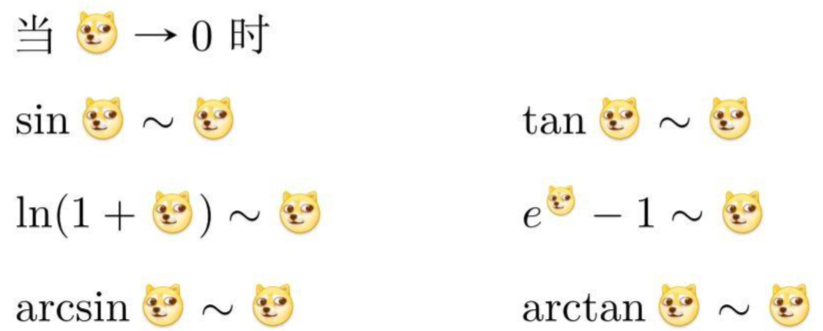
\includegraphics[scale=.45]{./Pics/Fomular1.png}
    \caption{等价无穷小替换}
    \label{等价无穷小替换}
\end{figure}


% \clearpage
我们使用一张下面的SVG矢量图片来进行公式的表达:
\begin{figure}[!htb]
    \centering
    \includesvg[scale=.3]{./Pics/Doge.svg}
    \caption{主人公Doge图示}
    \label{Doge}
\end{figure}


\newcommand{\doge}{\lower1.5pt\hbox{\scale{.03}{\includesvg{./Pics/Doge.svg}}}}
下面给出这个公式的矢量图版本:\doge 的演示如下:

常见的等价无穷下替换如下,当 \doge  $\to\; 0$ 时,我们恒有以下的式子成立:
\begin{align*}
    & \sin(\doge^2) \sim \doge                      && \tan(\doge)\sim \doge \\
    & \ln(1+\doge)\sim \doge                        && {\rm e}^{\doge} -1 \sim \doge\\
    & \arcsin(\doge) \sim \doge                     && \arctan(\doge) \sim \doge \\
    & \log_a(1+\doge) \sim \frac{\doge}{\ln a}      && \doge - \ln(1+\doge)\sim \frac{1}{2}\doge^2\\
    & 1-\cos(\doge) \sim \frac12\doge^2             && \ln(\doge + \sqrt{1+\doge^2}) \sim \doge \\
    & \doge -\sin(\doge) \sim \frac16\doge^3        && \tan(\doge)-\doge \sim \frac13\doge^3 \\
    & (1+\doge)^\alpha-1 \sim \alpha\doge           && \arcsin(\doge) -\doge \frac16 \doge^3\\
    & \doge - \arctan(\doge) \sim \frac13 \doge^3   && \tan(\doge) -\sin(\doge) \sim \frac12 \doge^3
\end{align*}

\clearpage
\subsection{Emoji编译}
说回正题,如果你想要使用彩色的表情包Emoji,那么目前的唯一选择就是:
% \noindent\rule{.9\linewidth}{2pt}
{\bf Lua\LaTeX}{\bf + Emoji宏包},具体的使用流程如下\emoji{ledger}:

\begin{itemize}
    \item \emoji{diamond-with-a-dot} 首先便是在导言区使用命令\verb|\usepackage{emoji}|
    \item \emoji{diamond-with-a-dot} 设置emoji对应的字体(Windows不用设置),
        Linux可以安装Twemoji Mozilla字体,不然的话,编译出来的pdf中表情包是位图。
    \item \emoji{diamond-with-a-dot} 然后编译方式改为 LuaLaTeX
\end{itemize}

至于怎么使用\emoji{face-with-monocle},直接参看增祥东老师写的官方文档:\verb|texdoc emoji|即可
\emoji{smiling-face-with-sunglasses}.

此时我们便可以使用Emoji编辑一个数学题了,一个emoji编辑的数学题如下:

\newcommand{\apple}{\mbox{\emoji{red-apple}}}
\newcommand{\banana}{\mbox{\emoji{banana}}}
\newcommand{\pear}{\mbox{\emoji{pear}}}
\begin{align}
\left\{
\begin{aligned}
    & 2\times\apple  - \pear + 3\times \banana = 10\\
    & 4\times\apple + 2\times\pear - 4\times\banana = -10 \\
    & \apple + \pear + \banana = 5
\end{aligned}
\right.
\end{align}

你还可以尝试一下下面这个题目,关于数论中整数的问题:

\begin{tcolorbox}[colframe=black,colback=white]
    95\% 的人解不出这道题!
    \begin{align}
        \frac{\apple}{\banana+\pear} 
            + \frac{\banana}{\apple+\pear} 
            + \frac{\pear}{\apple+\banana}
        = 4
    \end{align}

    你能找到 \apple, \banana, \pear 的整数解吗?
\end{tcolorbox}

\begin{warning}
    \emoji{warning}警告:这是一个钓鱼题目,别怪我们有告诉你。

    正确答案如下:
    \begin{align*}
        & a=154476802108746166441951315019919837\\
            &\hspace*{2em} 485664325669565431700026634898253202035277999\\
        & b=368751317941299998271978115652254748\\
            &\hspace*{2em} 25492979968971970996283137471637224634055579\\
        & c=437361267792869725786125260237139015\\
            &\hspace*{2em} 2816537558161613618621437993378423467772036
    \end{align*}
\end{warning}
                                                                                                                                                                                                                                                                                                         

\clearpage
\section{中英文字体设置}
\subsection{字体族声明}
中英文的字体族声明方式是不同的,下面是二者声明的方式:
\begin{lstlisting}
% 西文字体
\newfontfamily{\FamilyMame1}[Path=./Fonts/]{FontName1.ttf}
% 中文字体
\setCJKfamilyfont{FamilyName2}[Path=./Fonts/]{FontName2.TTF}
% 表情包字体
\newfontfamily{\EmojiFontFamily}[Path=./Fonts/]{FontName3.ttf}
\end{lstlisting}

从上面我们可以看出二者的声明是不同的,对应的二者的使用方法也不同:
\begin{lstlisting}
% 英文的使用
{\FamilyMame1  Your Text Here!}
% 中文的使用
{\CJKfamily{FamilyMame2} 你的文字内容}
% Emoji的使用
{\FamilyMame3  Your Emoji Here!}
\end{lstlisting}

很有可能你会遇到你自己定义的字体族无法加粗的问题,也就是说下面的对文中的中(日韩)文字语句无效:

\emoji{frog} 下面就是实际的演示情况

\verb|\textbf{\ComicA Hello你好}| \faLongArrowAltRight \;\textbf{\ComicA Hello你好},
\;\verb|{\bf Hello你好}| \faLongArrowAltRight \;{\bf Hello你好}

\verb|\textit{\ComicA Hello你好}| \faLongArrowAltRight \;\textit{\ComicA Hello你好},
\;\verb|{\it Hello你好}| \faLongArrowAltRight \;{\it Hello你好}

而且直接产生了如下的警告:

\noindent\rule{.9\linewidth}{2pt}
\begin{verbatim}
    Font shape `TU/comic.ttf(0)/bx/n' undefined
    (Font)	using `TU/comic.ttf(0)/m/n' instead. 

    Font shape `TU/comic.ttf(0)/m/it' undefined
    (Font)	using `TU/comic.ttf(0)/m/n' instead.
\end{verbatim}

其实上面的内容就是告诉你,你自己定义的字体族中的字体系列(加粗),字形(斜体)还没有指定。
此时你应该重新声明一下你自定义字体族的{\bf 字体系列},指定它的各种系列对应的字体,如下:
\clearpage
\begin{lstlisting}
\newfontfamily{\comicB}{comic.ttf}[
    BoldFont=comicbd.ttf,
    ItalicFont=comici.ttf,
    BoldItalicFont=comicz.ttf
]
\end{lstlisting}

再次测试一下,此时就能够对comic字体实现加粗了

\verb|\textbf{\ComicB  comic Bold font 你好}| \faLongArrowAltRight \;\textbf{\ComicB  comic Bold font 你好},

\verb|\textit{\ComicB  comic italic font 你好}| \faLongArrowAltRight \;\textit{\ComicB comic italic font 你好},

\begin{warning}
\emoji{keycap-1}\; 字体族,字体系列,字形,中文字体这几个概念是不同的,不知道的自己去百度.

\emoji{keycap-2}\; comic字体是给西文设置的,所以对中文才没有起作用.

\emoji{keycap-3}\; 西文才有字形概念,中文所谓的斜体概念都是word这个毒瘤产生的
\end{warning}


其实自己定义的字体族你还可以定义很多的东西,比如颜色,下面这个命令
定义了一个叫做ComicBlue的字体族,颜色默认是蓝色.
\begin{lstlisting}
\newfontfamily{\ComicBlue}[Path=./Fonts/]{comic.ttf}[Color=blue]
\end{lstlisting}

\verb|{\ComicBlue Blue Comic Font}| \faLongArrowAltRight\; {\ComicBlue Blue Comic Font}

 同样的,对于字体的加粗和斜体你可以偷懒,使用如下的命令声明
一个名为AutoF的字体族,它会自动同时实现中英文伪粗体和伪斜体,不用你自己单独去指定:
\begin{lstlisting}
\setCJKfamilyfont{AutoF}{FZSTK.TTF}[AutoFakeBold, AutoFakeSlant]    
\end{lstlisting}

演示效果:\verb|{\CJKfamily{AutoF}\bfseries 你好Hello}| \faLongArrowAltRight {\CJKfamily{AutoF}\bfseries 你好Hello}


局部的数学字体声明也是简单的,命令如下:
\begin{lstlisting}
% 设置数学公式字体,注意:三个选项设置中间不能有空格
\setmathfont(Digits, Greek, Latin){comic.ttf}
\setmathfont(Digits,Greek,Latin)[
    ItalicFont=comici.ttf,
    BoldFont=comicbd.ttf,
    BoldItalicFont=comicz.ttf
]{comic.ttf}
% 注意:如果没有给出新的数学字体的粗体和斜体
% 的样式的话,LaTeX会给出警告
\end{lstlisting}



\clearpage
\section{全局}
\subsection{正文字体}
\emoji{face-with-monocle} 也许你会遇到这样一种情况,我使用下面的命令改变了全文的西文字体后,
中文根本就没有变,那么问题出在哪里了??
\begin{lstlisting}
    \setmainfont{Times New Roman}
\end{lstlisting}
西文字母和中文的全局声明固然不同,西文和中文的设置命令如下:
\begin{itemize}
    \item \verb|\setmainfont{Times New Roman}| \faLongArrowAltRight 设置全局西文字体为Times New Roman
    \item \verb|\setCJKmainfont{STKAITI.TTF}| \faLongArrowAltRight 设置全文的中文字体为楷体
\end{itemize}


下面是一个完整的设置全文中英文字体示例
\begin{lstlisting}
\setmainfont{comic.ttf}
% 先清空中文字体设置,再重新设置中文字体
\renewcommand\CJKrmdefault{}
\setCJKmainfont{STKAITI.TTF} 
\end{lstlisting}

具体的演示效果如下:
\begin{figure}[!htb]
    \centering
    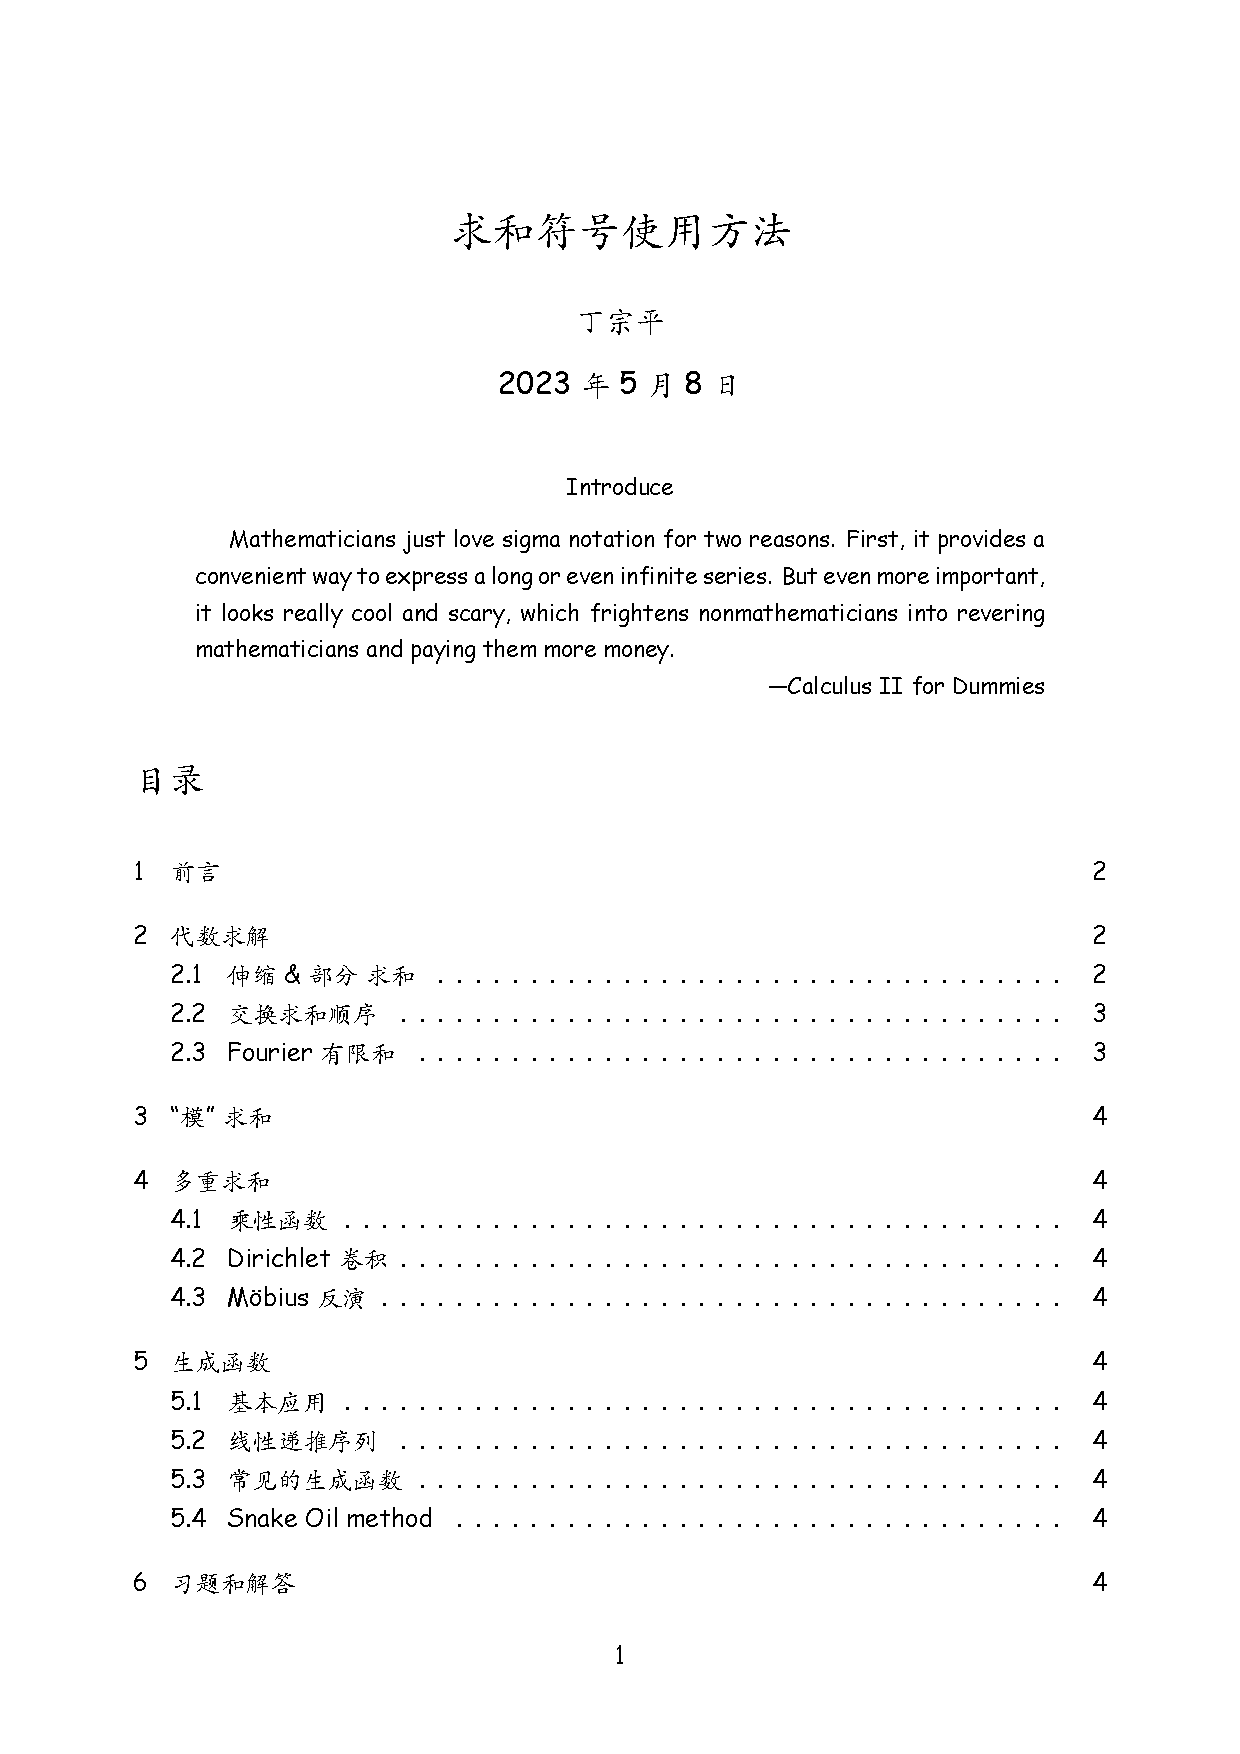
\includegraphics[width=.23\linewidth]{./Pics/p1.pdf}
    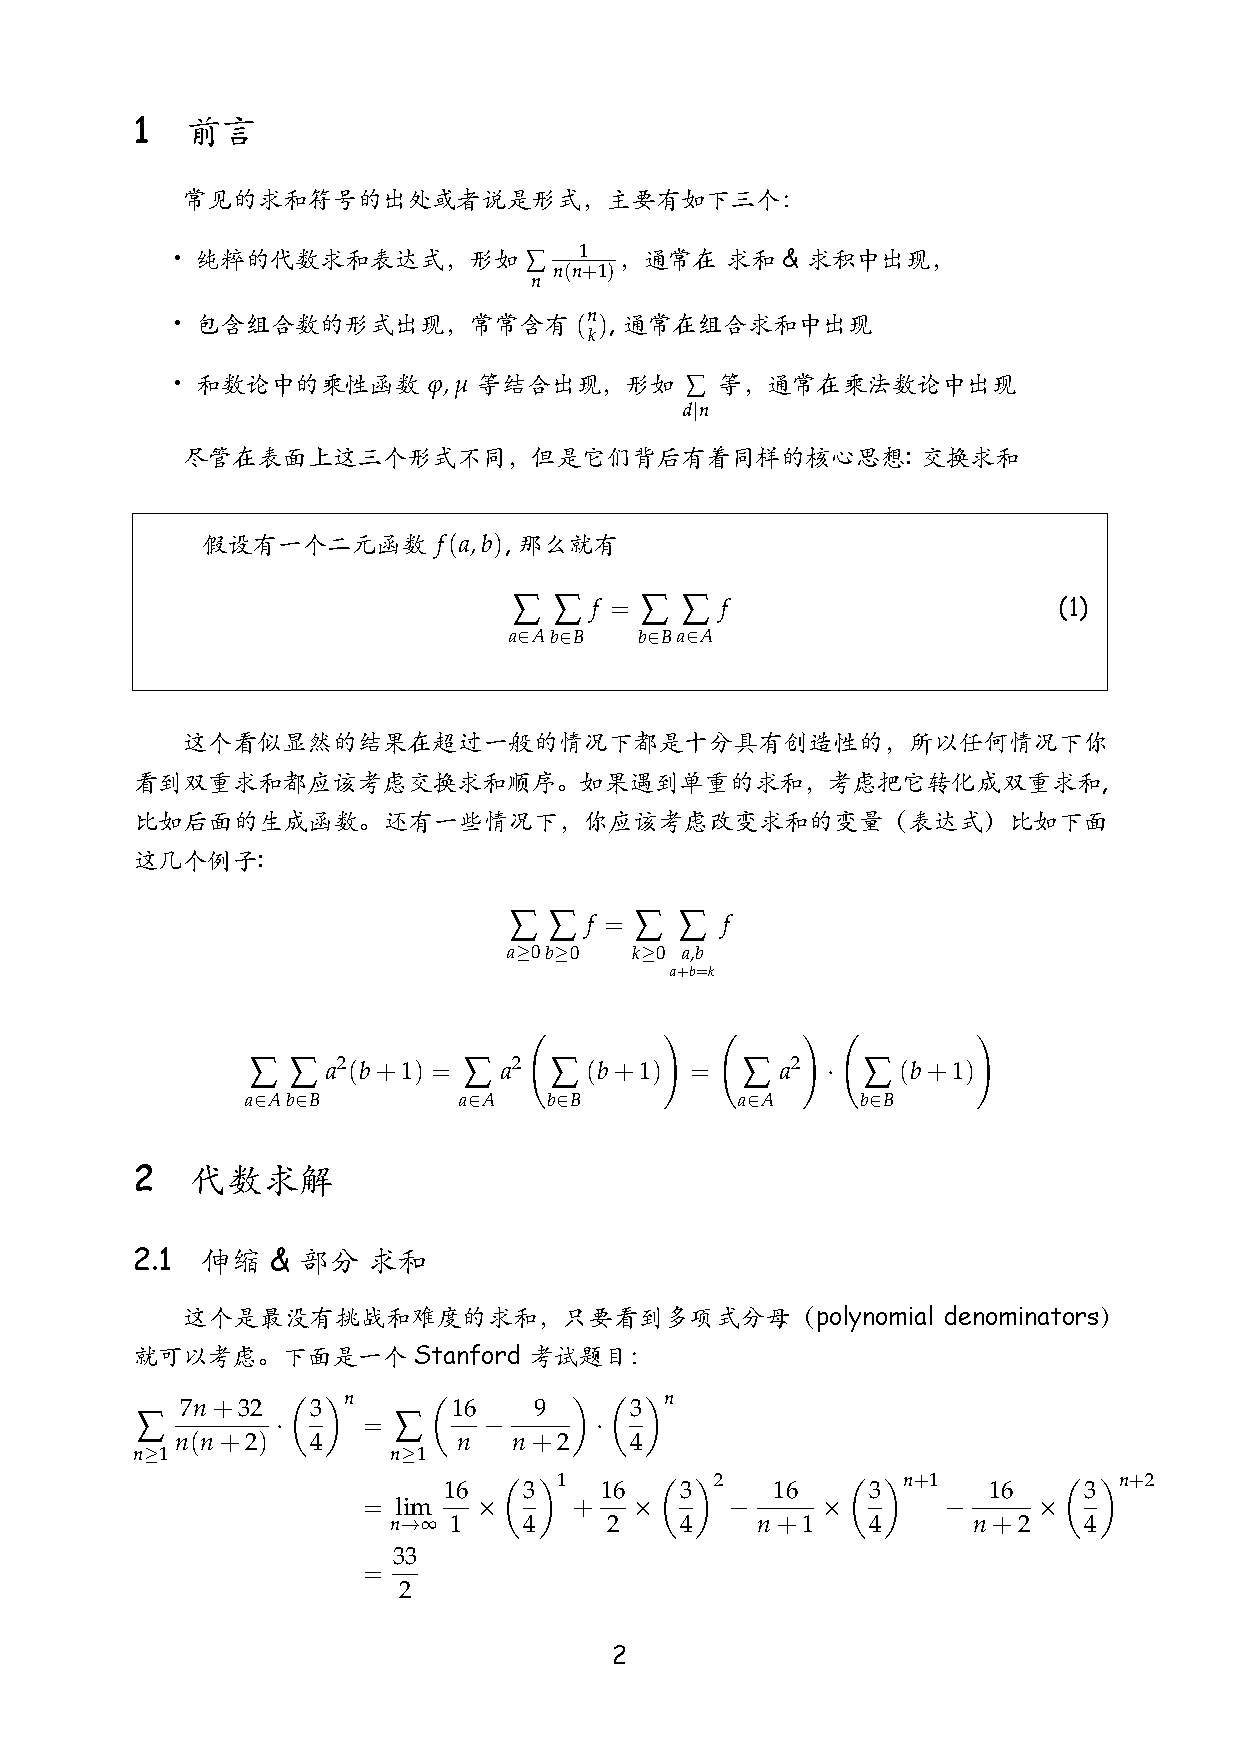
\includegraphics[width=.23\linewidth]{./Pics/p2.pdf}
    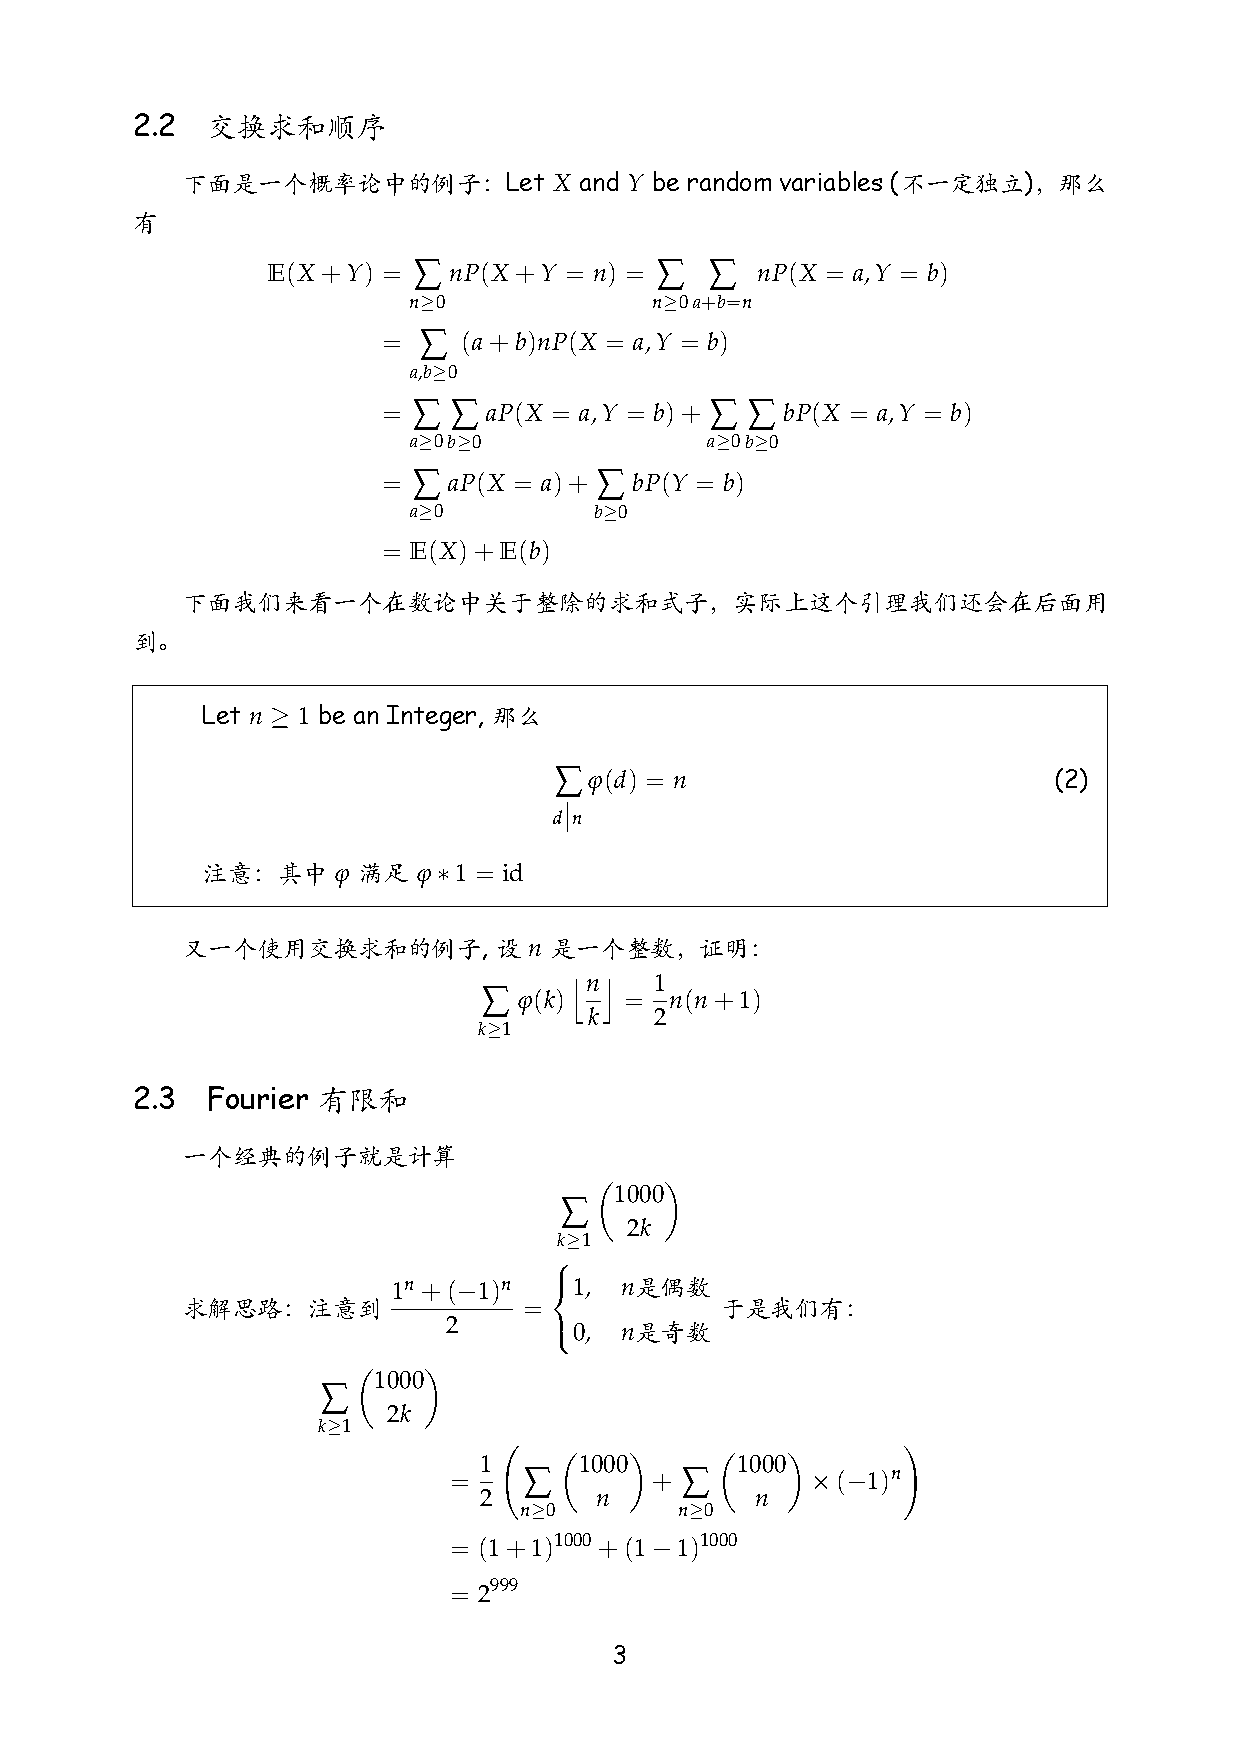
\includegraphics[width=.23\linewidth]{./Pics/p3.pdf}
    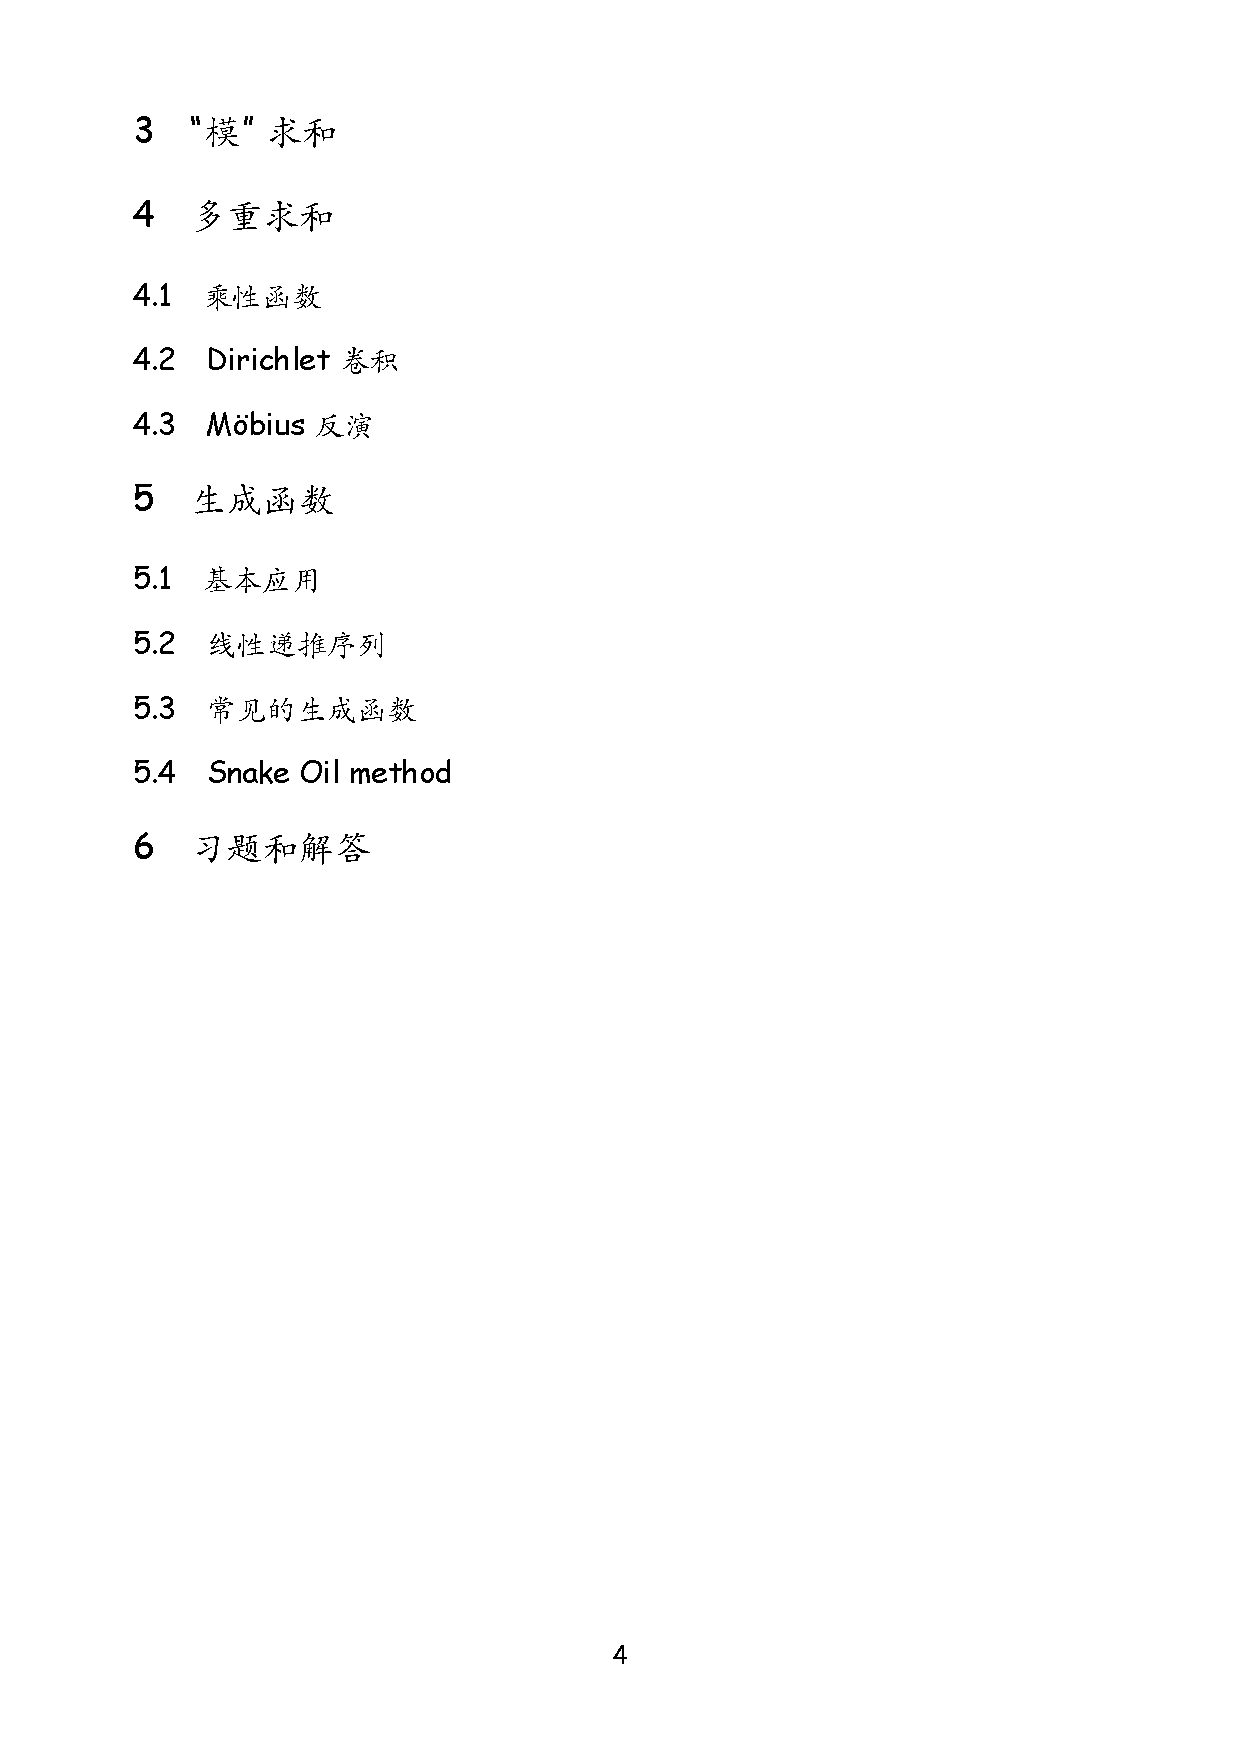
\includegraphics[width=.23\linewidth]{./Pics/p4.pdf}
    \caption{全局字体设置}
    \label{全局字体设置}
\end{figure}

当你设置了font的Path后,更加的简单:
\begin{lstlisting}
\setCJKmainfont[
    Path = fonts/zh_CN-Adobe/,          % 设置字体的路径
    Extension = .otf,                   % 扩展名设置,省略扩展名
    BoldFont=AdobeHeitiStd-Regular,     % 粗体设置
    ItalicFont=AdobeKaitiStd-Regular,   % 斜体设置
    SmallCapsFont=AdobeHeitiStd-Regular % 小型大写字体
    ]{AdobeSongStd-Light}
\end{lstlisting}

\begin{warning}
\emoji{keycap-1}\; 本来{\sffamily \TeX}这玩意儿就是为了西文发明的,也就能理解对亚洲文字支持差

\emoji{keycap-2}\; 在当今的形势下,使用英语是必须的,慢慢的习惯,然后其实还挺好的,关键是{\ttfamily \LaTeX}的编译速度,使用方便程度会指数式上升。
\end{warning}



% \clearpage
\subsection{数学字体}
{\ttfamily \LaTeX}中的数学字体又是一个大坑,尽管我们的{D.E. K} 在最开始设计
{\ttfamily \TeX}的时候就为它设计了一个Computer Modern字体,{\ttfamily \LaTeX}
中的数学字体可以分为如下的几类:
\begin{itemize}
    \item \emoji{diamond-with-a-dot} 原生为 {\ttfamily \TeX} 设计的:
        Computer Modern, CM Bright, Concrete and Euler, Concrete Math,
        Iwona, Kurier, Antykwa Półtawskiego, Antykwa Toru\' nska
    \item \emoji{diamond-with-a-dot} Core Postscript Fonts核心字体系列:
        Kerkis, Millennial, fouriernc, pxfonts, Pazo, mathpple, txfonts, Belleek,
        mathptmx, mbtimes
    \item \emoji{diamond-with-a-dot} 后面设计的一些免费的数学字体:
        Arev Sans, Math Design with Charter, Math Design with Garamond,
        Fourier-GUTenberg, Math Design with Utopia
\end{itemize}

注:绿色盒子的tcolorbox定义
\begin{lstlisting}
% \usepackage{tcolorbox}
% \tcbuselibrary{skins}
\newtcbox{\mathfontname}{
    enhanced,nobeforeafter,
    % 边距
    tcbox raise base,boxrule=0.4pt,
    top=0mm,bottom=0mm,
    right=0mm,left=4mm,
    arc=1pt,boxsep=2pt,before upper={\vphantom{dlg}},
    % 颜色
    colframe=green!50!black,
    coltext=green!25!black,
    colback=green!10!white,
    overlay={
        \begin{tcbclipinterior}
            \fill[green!75!blue!50!white] (frame.south west)
                rectangle node[
                        text=white,
                        font=\sffamily\bfseries\tiny,rotate=90
                ] 
                {Font} ([xshift=4mm]frame.north west);
        \end{tcbclipinterior}}}
\end{lstlisting}

\emoji{electric-plug}\; 先看下{\ttfamily \LaTeX}中默认的数学字体,word中常用的
Cambridge Math Font字体以及书籍中常用的Euler Math Font字体:

\begin{center}
    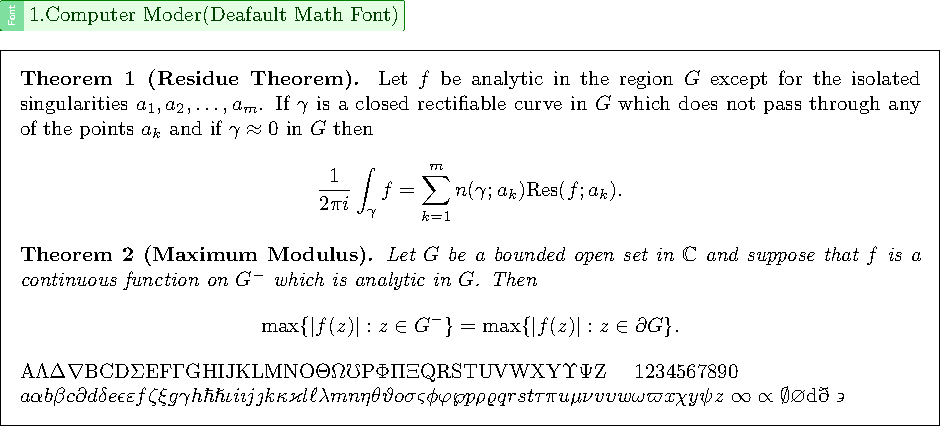
\includegraphics[width=.95\linewidth]{./MathFontVision/Computer-Modern.pdf} 

    \vspace*{2em}
    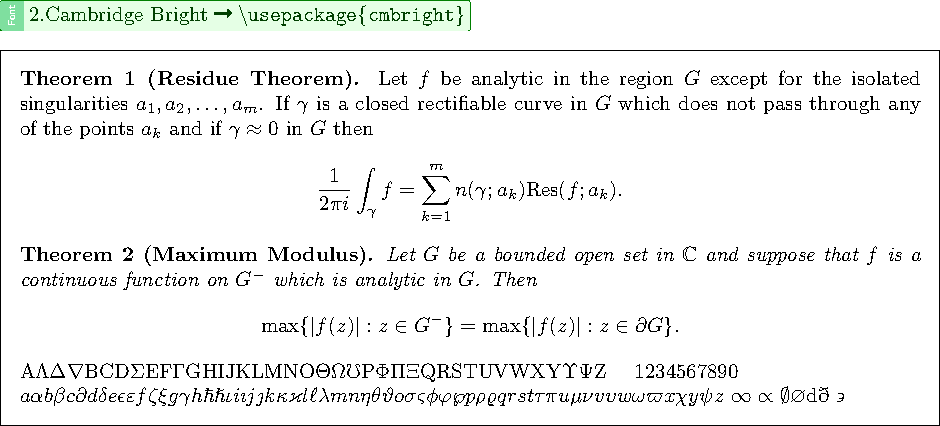
\includegraphics[width=.95\linewidth]{./MathFontVision/CmBright.pdf} 

    \vspace*{2em}
    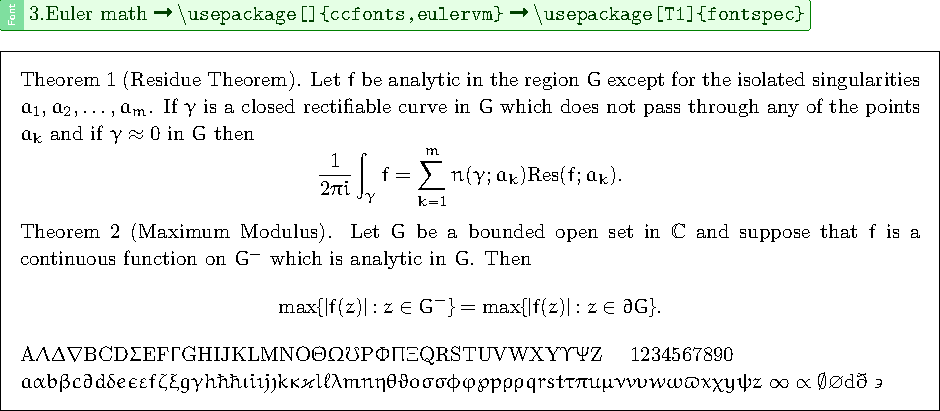
\includegraphics[width=.95\linewidth]{./MathFontVision/Euler-Math-Font.pdf} 
\end{center}

\clearpage
\emoji{electric-plug}\; 后面便是其他的Core Postscript Fonts数学字体
\begin{figure}[!htb]
    \centering
    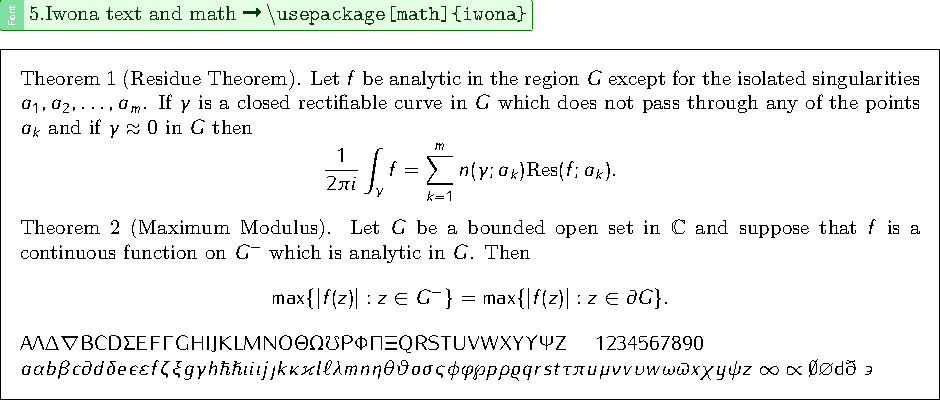
\includegraphics[width=.95\linewidth]{./MathFontVision/Iwona-Text-and-Math.pdf}
    
    \vspace*{2em}
    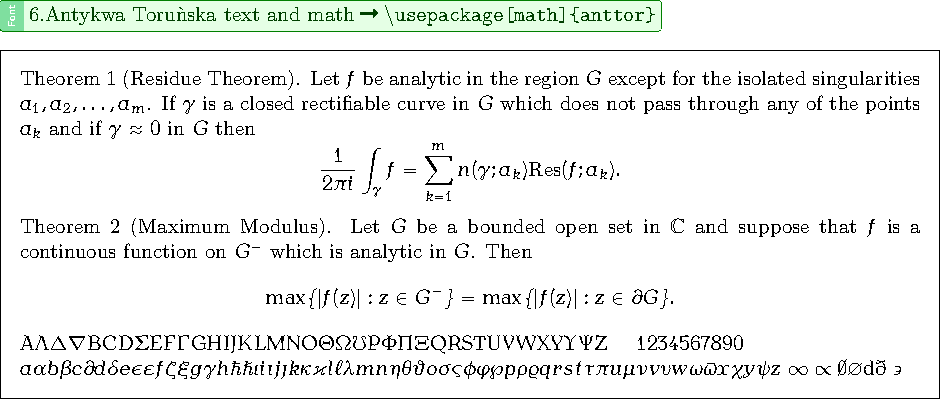
\includegraphics[width=.95\linewidth]{./MathFontVision/Antykwa-Torunska-Text-and-Math.pdf}

    \vspace*{2em}
    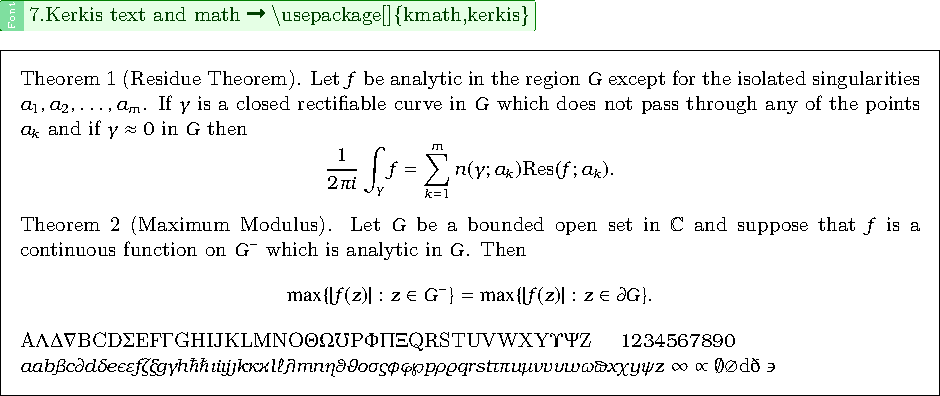
\includegraphics[width=.95\linewidth]{./MathFontVision/Kmath-Kerkis-Text-and-Math.pdf}
\end{figure}


\begin{figure}[!htb]
    \centering
    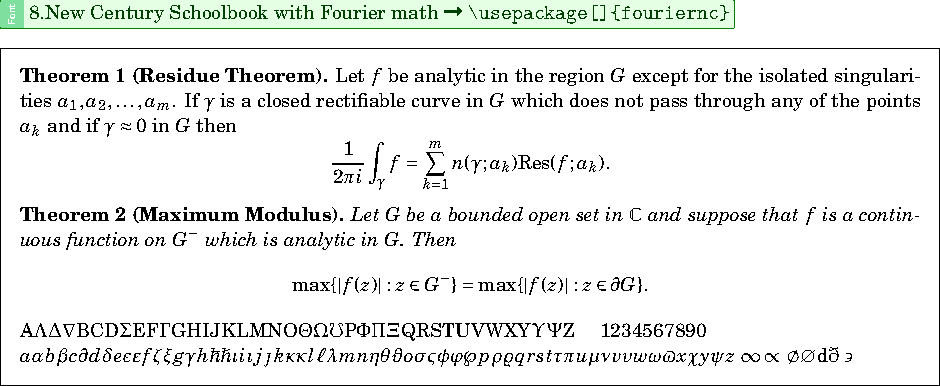
\includegraphics[width=.95\linewidth]{./MathFontVision/New-Century-Schoolbook-with-Fourier-Math.pdf}
    
    \vspace*{2em}
    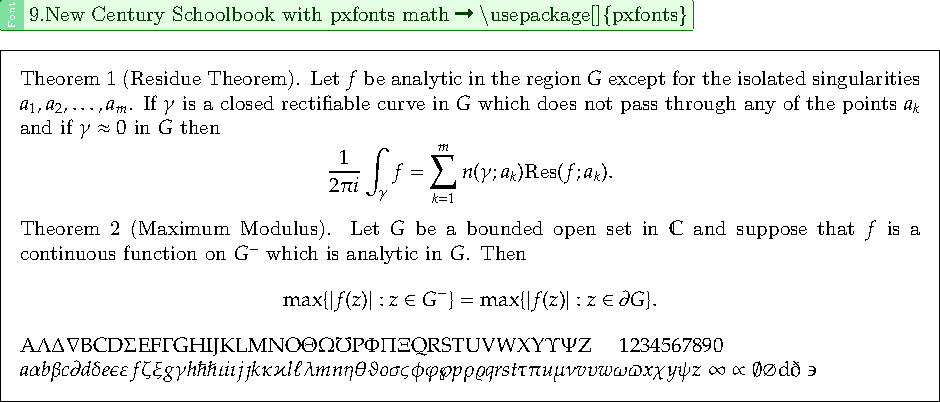
\includegraphics[width=.95\linewidth]{./MathFontVision/New-Century-Schoolbook-with-Pxfonts-Math.pdf}
    
    \vspace*{2em}
    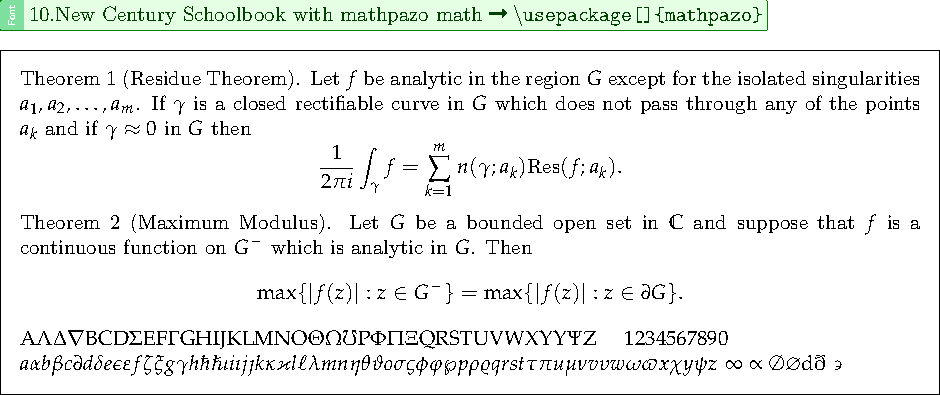
\includegraphics[width=.95\linewidth]{./MathFontVision/New-Century-Schoolbook-with-Mathpazo-Math.pdf}
\end{figure}


\begin{figure}[!htb]
    \centering
    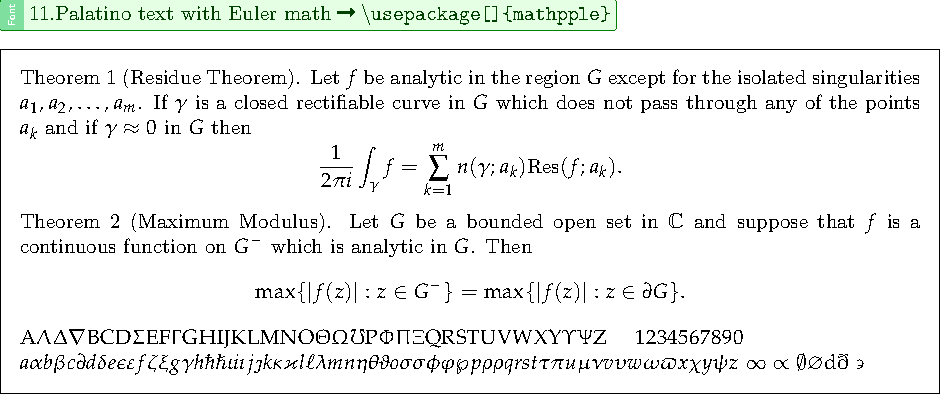
\includegraphics[width=.95\linewidth]{./MathFontVision/Palatino-Text-with-Euler-Math.pdf}

    \vspace*{2em}
    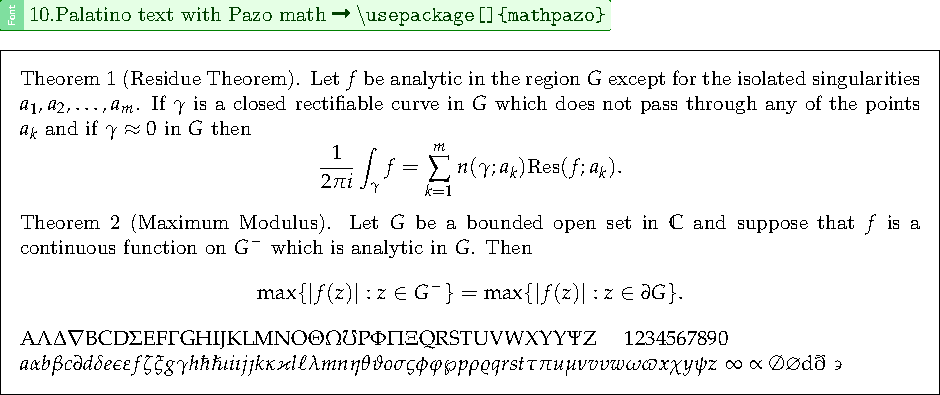
\includegraphics[width=.95\linewidth]{./MathFontVision/Palatino-Text-with-Pazo-Math.pdf}
    
    \vspace*{2em}
    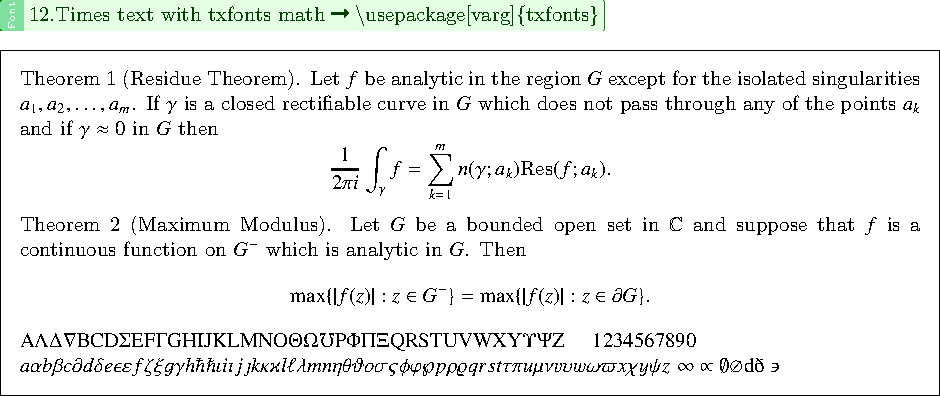
\includegraphics[width=.95\linewidth]{./MathFontVision/Times-Text-with-Txfonts-Math.pdf}
\end{figure}


\clearpage
\emoji{electric-plug}\;其它的一些免费的数学字体,如下:
\begin{figure}[!htb]
    \centering
    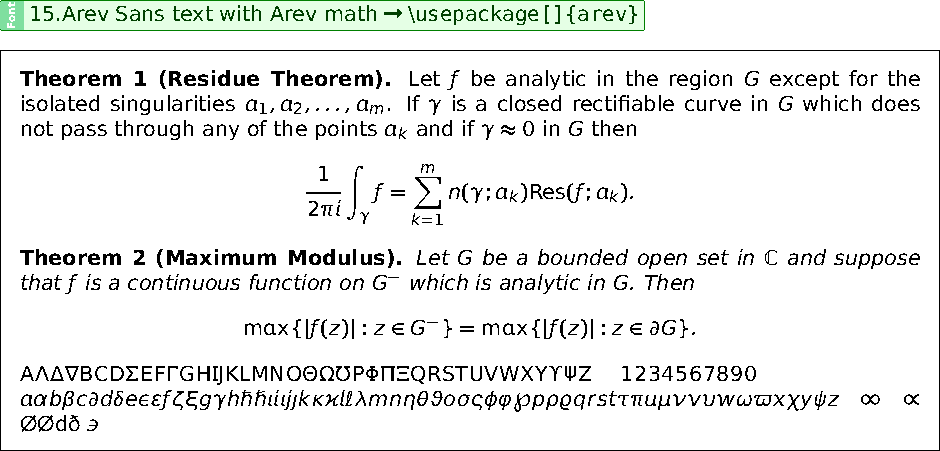
\includegraphics[width=.95\linewidth]{./MathFontVision/Arev-Sans-Text-with-Arev-Math.pdf}

    \vspace*{2em}
    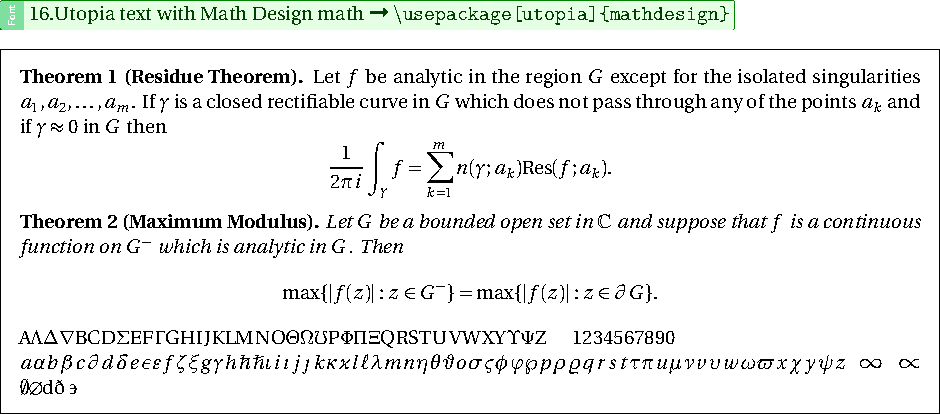
\includegraphics[width=.95\linewidth]{./MathFontVision/Utopia-Text-with-Math-Design-Math.pdf}
\end{figure}


\section{结语}
\begin{center}
    \scale{8}{\FathonyKing Thank you} 
\end{center}



\end{document}
